<<<<<<< HEAD
% This is samplepaper.tex, a sample chapter demonstrating the
% LLNCS macro package for Springer Computer Science proceedings;
% Version 2.20 of 2017/10/04
%
\documentclass[runningheads]{llncs}
%
\usepackage{graphicx}
\usepackage{hyperref}
\renewcommand\UrlFont{\color{blue}\rmfamily}
=======

\documentclass{IOS-Book-Article}

\usepackage{mathptmx}
\usepackage{soul}\setuldepth{article}
<<<<<<< HEAD
\usepackage{booktabs}
=======
 
>>>>>>> 7c1cec024806f0122dbd3ebada2b3244dc9de7ab
%\usepackage{times}
%\normalfont
%\usepackage[T1]{fontenc}
%\usepackage[mtplusscr,mtbold]{mathtime}
%
<<<<<<< HEAD
\def\hb{\hbox to 10.7 cm{}}
=======
\usepackage{graphicx}
\usepackage{hyperref}
%\renewcommand\UrlFont{\color{blue}\rmfamily}
>>>>>>> c5f4a12... Mise a jour Method
\setlength{\parskip}{0pt}
\raggedbottom
\usepackage{multirow}
\usepackage{amsmath}
\usepackage{csquotes}
\usepackage{paralist}
\usepackage{booktabs}
\usepackage{mathptmx}
<<<<<<< HEAD
=======
>>>>>>> 7c1cec024806f0122dbd3ebada2b3244dc9de7ab
>>>>>>> c5f4a12... Mise a jour Method
\usepackage{pgfplots}
\pgfplotsset{compat=1.8}
\usepackage{subfigure}
\pgfplotsset{width=7cm,compat=1.8}
\usepackage{pgfplotstable}
<<<<<<< HEAD
\renewcommand*{\familydefault}{\sfdefault}
\usepackage{tikz}

\begin{document}
\title{Prediction of Malaria with Machine Learning Algorithms : An experimental Study}

%%
%% The "author" command and its associated commands are used to define
%% the authors and their affiliations.
%% Of note is the shared affiliation of the first two authors, and the
%% "authornote" and "authornotemark" commands
%% used to denote shared contribution to the research.
\author{Ousseynou Mbaye \and Mouhamadou Lamine Ba  \and Alassane Sy}
%
\authorrunning{Ousseynou Mbaye \and M. Lamine Ba  \and Alassane Sy}
% First names are abbreviated in the running head.
% If there are more than two authors, 'et al.' is used.
%
\institute{Universit\'e Alioune Diop de Bambey, Bambey, Senegal\\
\email{firstmidlle.last@uadb.edu.sn}
}



%%
%% By default, the full list of authors will be used in the page
%% headers. Often, this list is too long, and will overlap
%% other information printed in the page headers. This command allows
%% the author to define a more concise list
%% of authors' names for this purpose.
%\renewcommand{\shortauthors}{O. Mbaye et al.}

%%
%% The abstract is a short summary of the work to be presented in the
%% article.

%%
%% The code below is generated by the tool at %%http://dl.acm.org/ccs.cfm.
%% Please copy and paste the code instead of the example below.
%%


%%
%% Keywords. The author(s) should pick words that accurately describe
%% the work being presented. Separate the keywords with commas.



%
\maketitle              % typeset the header of the contribution
%
\begin{abstract}

Still today, Malaria remains one of the most feared diseases in Sub- Saharan Africa and especially in Senegal. This is mainly due to inappropriate medical care support coupled with an often late and error-prone diagnosis from the medical staff. In addition, largely used diagnostic standards such as the Rapid Diagnosis Test is not fully reliable. With the development and increasing adoption of automated tools in the health field, machine learning applications might help medical actors in their decision-making process. In this paper, we propose an experimental study of six machine learning algorithms for the prediction of Malaria in Senegal. These algorithms aim at predicting whether or not a given patient suffers from Malaria based on his signs and symptoms. The performance of the algorithms have been extensively tested and evaluated over real data sets about patients in Senegal that suffer or not from Malaria. The algorithms are evaluated using four criteria: accuracy, Recall, F-measure, Precision and Specificity. The research has shown that there is not necessarily a single best classification tool, but instead the best performing algorithm will depend on the dataset to be analysed
 
\end{abstract}
%
%
% Introduction
\section{Introduction}\label{intro}
Malaria is one amongst the most deadly disease in the world, especially in sub-saharan Africa countries such as Senegal.
Malaria is caused by parasitic single-celled microorganisms belonging to the Plasmodium group; it is an infectious
disease which is transmitted to human being through bites from infected female Anopheles mosquitoes. Someone who suffers
from  Malaria may present symptoms that typically include fever, tiredness, vomiting, and headaches. In its severe form,
the disease can cause yellow skin, seizures, coma or death.

\subsubsection{Studied problem and motivations.}
According to the last report \cite{Wh17}  about the propagation of Malaria disease around the world, published in November 2017 by the World international Health Organization (WHO in short),
 216 millions of cases have been reported in 2016. As a result, the number of cases has significantly increased when compared to the 211 millions of reported Malaria patients in 2016.
As for the number of death due to Malaria, it does not decrease between 2016 and 2017 (446.000 vs. 445.000) despite the huge effort made by governements
and non-governmental organization to improve healthcare services and the awareness strategies, especially in critical areas. 
When analyzing the statistics above in details, one can easily notice that the burden of the Africa region of the World 
international Health Organization is colossal. Indeed, 90\% of Malaria cases and 90\% of deaths due to the disease were located in this area in 2016.
More specifically, 80\% of the burden in terms of morbidity is distributed in fifteen countries, all located in Sub-saharan Africa except India. This demonstrates
that Malaria is a real flail in Sub-saharan Africa states and Senegal is not spared at all. We investigate in this study an efficient approach to predict, using machine learning, the occurence 
or not of Malaria when a patient has to be diagnosed. Given the patient signs and symptoms, as well as the result from the quick diagnosis test, our solution should be to 
automatically tell if she suffers from Malaria or not with a high accuracy.

Malaria is an acute problem in Senegal  due mainly to the lack of high quality healthcare services and well-formed
staffs able to perform accurate diagnosis of diseases that patients suffer from. Over the past years, the government with 
the help of international organizations have tried to eradicate Malaria by implementing various proactive and reactive solutions 
to fill the gap in terms of services and human resources. However, the mortality rate is still very high, e.g. in underserved areas,
areas without required healthcare needs, uneducated people, population with low income, etc. Most of these deaths cases are reported to be caused by inaccurate diagnosis, sometimes 
incomplete leading to a bad prediction of the exact type of Malaria.
On the other hand, Malaria occurence or complication can often occur during  popular events (for instance religious events such as the Grand Magal of Touba \cite{So17})
which gather thousands of persons from everywhere in the country during a short time period. During those popular events, non-permanent medical points are set in order
to assist and treat ill persons; the staff in a given health point might be formed sometimes by only volunteers without advanced medical skills. Each of these medical 
points might receive and treat hundreds of patients each day with some of them potentially suffering from Malaria. 
This appeals for the need of finding automated tools to help medical actors in their decision making process, and thereby to improve provided 
healthcare services.   

\subsubsection{Proposed diagnosis approach.}
In this paper we present first steps towards an efficient manner to automatically diagnosis Malaria occurence or not based on patient signs and symptoms,
and the outcome from the quick diagnosis test. We define our diagnosis task as a classical binary classification problem by considering two classes: \textquote{Malaria} and \textquote{not-Malaria}.
Given a patient data, our main goal is to properly find to which class the patient belongs. To solve this classification problem we rely on machine learning and use the logistic regression
function as the basis of our prediction approach. Machine learning has been largely used in several domains (e.g. Health Informatics  \cite{Du13}) for various purposes whereas logistic regression has demonstrated its efficiency when dealing with a binary classification problem. 
 
As an application scenario, we focus on predicting Malaria cases in Senegal. At this end, we use  a large volume of patient record dataset collected during the most popular religious event in Senegal from the different installed health points, namely more than twenty points that deadly receive hundreds of patients.
As an immediate result of this work, we introduce a data preparation pipeline in order to 
\begin{inparaenum}[(i)]
\item explore the dataset for profiling purpose;
\item only retain records related to Malaria;
\item clean and transform attributes, as well data values, into the extracted Malaria dataset; and 
\item impute missing values (there were lot of missing values in the collected health dataset as reported in Section\ref{data_prep}).
\end{inparaenum}
Such a data preparation pipeline has been realized using \emph{OpenRefine} (formely Google Refine) to perform various cleaning and profiling tasks on our raw atient dataset and \emph{missForest}, a robust
 algorithm for imputing  missing data of diverses types; see Section \ref{data_prep} for more details. 
Expermients on the real world patient dataset, augmenting with a semi-synthetic dataset, show promising performance results regarding the effectiveness of the proposed approach.

\subsubsection{Paper organization.}The remaining of the paper is organized as follows. We summarize the related work on data imputation and binary classification methods in Section \ref{related_work}.
In Section \ref{data_prep} we introduce a data preparation pipeline on the raw collected patient records for the prediction phase. 
We then present our prediction model for Malaria cases in Section \ref{prediction_model}.
Experiments and performance analysis  on the collected real-world dataset, as well as a semi-synthetic dataset,  are detailled in Section \ref{experimentation} before we conclude in Section \ref{conclusion}. 


% Prediction Model
\section{Review of evaluated ML algorithms}\label{ml_algorithms}
We considered and comparatively evaluated  the performance of six machine learning algorithms for the task of predicting Malaria appearance for patients living in Senegal. Those algorithms are chosen among the most used ones in the health field according to studies \cite{de2018binary,tomar2013survey}. In the following we briefly describe each of them.

% Naive Bayes
\textbf{ Naive Bayes classifier (NB) }\cite{Ka17} is a \emph{supervised} machine learning algorithm, i.e. requires to be trained, used for classifying observations to given distinct classes based on \emph{input explanatory variables} (a.k.a feature or attribute).
It is a classification technique based on the well-known \emph{Bayes’ theorem}\footnote{https://en.wikipedia.org/wiki/Bayes\%27\_theorem} with strong and naive assumptions.
It simplifies learning by assuming that features are independent of given class.

% Logistic Regression
 
\textbf{Logistic regression (LR)} \cite{Ph88} is a statistical model used in the machine learning domain as a supervised classifier for binary classification \cite{uddin2019comparing}. 
It is based, in its basic form, on a logistic function to describe a binary dependent variable\cite{wang2014support,de2018binary} by considering as input 
qualitative or/and ordinal explanatory variables  in order to measure the probability of a given class label. The greatest advantage  of the logistic regression
classifier is the fact that you can use continuous explanatory variables and it is easier to handle more than two explanatory variables simultaneously. One the other 
hand, the logistic regression is one of the most used multi-valued models in epidemiology.

% Decision Tree

\textbf{Decision tree (DT)} \cite{Ro05} is a supervised classifier which is obtained by recursively partitioning the labelled set of observations. It is one of the most adopted classifiers, thanks to its simplicity and its straightforward interpretation. For CART algorithms, hyperparameters are the impurity criteria (entropy and gini), the maximum depth, the minimum samples to split and the minimum samples at a leaf
 
% Random forest 

\textbf{Random Forest (RF)} \cite{Be01} is an ensemble approach built upon many decision tree classifiers. It is a supervised classifier which requires the same hyper parameters as DT, plus the number of trees to create and the random number of features
to look at when splitting the labelled data during the training step \cite{Be01}. 
%Support Vector Machine
 
\textbf{Support Vector Machine (SVM)} \cite{Ev01} is a supervised classification approach whose intuition is to represent input data in a space and to determine the optimal hyper-plane that divides that space in two regions depending on the targeted value.

% artificial neural networks

\textbf{An Artificial Neural Network (ANN)} \cite{Me19} is a computational approach also referred to as a Connectionist System used in Machine Learning. ANNs are loosely modeled after the biological neural network in an attempt to replicate the way in which we learn as humans. Think of it as a computing system, structured as a series of layers, each layer consisting of one or several neurons. The types of the layers comprise \emph{input}, \emph{output} and \emph{hidden} layers \cite{anderson1972simple,raschka2015python}.



% Related work
\section{Related work}\label{related_work}
In this section, we summarize the sate-of-the-art research on Malaria in general, and in particular the
use of machine learning techniques to tackle the various aspects related to one of the 
major healthcare problems worldwide which is Malaria.

% Studies on Malaria
As it is well-known, Malaria is caused by the bite of the female Anopheles, the most dangerous of which
is Plasmodium falciparum. Many early works have been consequently focused on the study of the evolution and
the distribution of the responsible mosquito, mainly with the goal to detect or diagnosis the severity of the 
disease given an infected patient \cite{Fe03,Al09}. Recent research on Malaria have largely adopted machine learning
and showed its ability to solve various aspects of the disease. Most of these machine learning based techniques are 
based on the analysis of blood data obtained from high-definition microscopic screenshots as in \cite{Ku18}. The authors
in \cite{Ku18} propose an unsupervised learning algorithm that detects and determines the types of infected blood cells.
Used prediction approach consists of quantifying the amount of plasmodium parasites in a blood smear. In the same research intuition
of harnessing blood, the Jordan-Elman neural network classifier introduced in \cite{Ha15}, on the other hand, to quickly determine the occurrence 
of Malaria and its severity level as well: the neural network analyzes the features of the blood data of the patients.  
Still using ML, DIAZ et al. have proposed in \cite{Dia09} a semi-supervised algorithm enable to quantify and classify the 
erythrocytes infected by Malaria parasistes through microscopic images. The orginiality of this work comes from its usability
even in the presence of thin blood drandruff infected by falciparum Plasmodium for the quantification and the classificationi tasks.
Besides blood data, sign and symptom records were also used to study Malaria with ML methods. Indeed, decision trees based approach
has been proposed in Nigeria \cite{Ug10} to predict the occurrence of Malaria given diagnostic data. However a decision tree suffers 
from various limitations as a classifier. Indeed it can easily overfit or can be extremely sensitive to small pertubations in data for instance.
Even though we both rely on signs and symptoms, the prediction model in \cite{Ug10} differs from ours on numerous facets: our model is built upon
logistic regression and is trained using also inputs from the quick diagnosis test. In addition, we apply our method in the context of patients living in Senegal. 
An example of previous work that has used logistic regression is that of Farida et al. in \cite{Ad10}. The logistic regression is exploited
there for the selection of features in order to construct stable decision trees. The decision trees are then used to predict the severity
criteria of Malaria in the context of Afghanistan. 


In the same line of works applying machine learning, in \cite{Pr17}, Pranav et al. propose Malaria likelihood prediction model built on a deep reinforcement learning (RL) agent. 
Such a RL predicts the probability of a patient testing positive for Malaria using answers from questions about their household. In 
the presented approach the authors have also dealt with the problem of determining the right question to ask next as well as the length of the survey, dynamically.
Moreover, statistically enhanced rule-based classification model to diagnose malaria has been proposed in \cite{Bb16}. A corresponding prototype 
which incorporates the rules and statistical models have been implemented; the main goal of the study was to develop a statistical 
prototype to perform clinical diagnosis of malaria given its adverse effects on the overall healthcare, yet its treatment remains 
very expensive for the majority of the patients to afford.

To the best of our knowledge this is the first work in Senegal that attempts to provide a prediction model for identifying 
the occurrence of Malaria given patient data.  


% Data Preparation
\section{REAL PATIENT HEALTH DATASETS}\label{datasets}
In order to carry out  our experiments in a real setting we have collected two real world datasets about patients living in Senegal. We describe each of them in the sequel.

\subsubsection*{\textbf{Data collection.}} Our first dataset, that we  to refer to it as DT1, contains medical records about patients living in distinct places in Senegal. It has been collected in 2016 during the \textquote{Grand Magal of Touba}  which is one of the most popular religious event in Senegal. Such an event gathers every year several millions of persons that come from various areas around the country \cite{Ch17}.  During the event several fixed and mobile health points are set up to enable the examination and treatment of ill persons. The second dataset, denoted by DT2, has been collected by drawing our attention on medical records about patients living in the same area. We focused on the district of Diourbel,Thies and Fatick \footnote{https://en.wikipedia.org/wiki/Diourbel\_Region} where the prevalence of Malaria is very high and collected patient records from its different health structures. 

\subsubsection*{\textbf{Data features. }} Table \ref{raw_data} contains the main characteristic of each dataset in terms of number of recorded variables (mainly clinical features), number of observations, variable types, number of observations per class (Malaria or Not Malaria), and the precision of the Rapid Diagnosis Test. In details, values for seventeen variables have been extracted for each observation in both datasets; two variables are basically of numerical types while the remaining are Boolean. Some of these variables (also called features or attributes) include personal data about the patient, but also signs and symptoms of the patient reported by the doctor who treated this later. The other attributes describe clinical data such as information about the doctor's final diagnosis (the patient's disease), the outcome of the Rapid Diagnosis Test and the patient's status (i.e. admission, death or observation). For privacy reasons and certain restrictions in the use of the data, we have ignored patient personal data  during this study.
In addition, we can observe that the first dataset is larger than the second one (21083 observations versus 5809 observations). Moreover, both datasets are unbalanced because the proportion of observations per class is largely unequal. As an example for dataset DT1 we have 614 observations in the first class and 5108 observation in the second class. Finally, we remarked that the precision of the Rapid Diagnosis Test is around 90\% for both datasets, meaning that
the systematically performed RDT in Senegal is not fully reliable.

On the other hand,  Figure \ref{missing_values} shows that the raw datasets come with missing values for  some variables on given observations.
To resolve the problem of unbalanced datasets and data messness, we followed a data preparation pipeline in order to fit our datasets into the good format for our experimentation; we discuss about such a data preparation step next. 

\begin{table*}[!ht]
\centering
  \begin{tabular}{cccccccc}
    \toprule
    \multirow{2}{*}{\textbf{Dataset}} &
      \textbf{Variables}&\textbf{Observations}&
      \multicolumn{2}{c}{\textbf{Variables types}}& \multicolumn{2}{c}{\textbf{Classes}} & \textbf{Precision of RDT}\\
    & & & Numeric & Boolean & Malaria & not Malaria \\
    \midrule
    DT1 &16 & 21083  & 2 &  14& 614&20469 & 90.23\% \\
    DT2 & 16 & 5809 & 2 & 14 & 5108&701 & 90.49\% \\
    \bottomrule
  \end{tabular}
  \caption{Raw Data characteristics}\label{raw_data}
\end{table*}
%
\begin{figure*}[!ht]
    \centering
    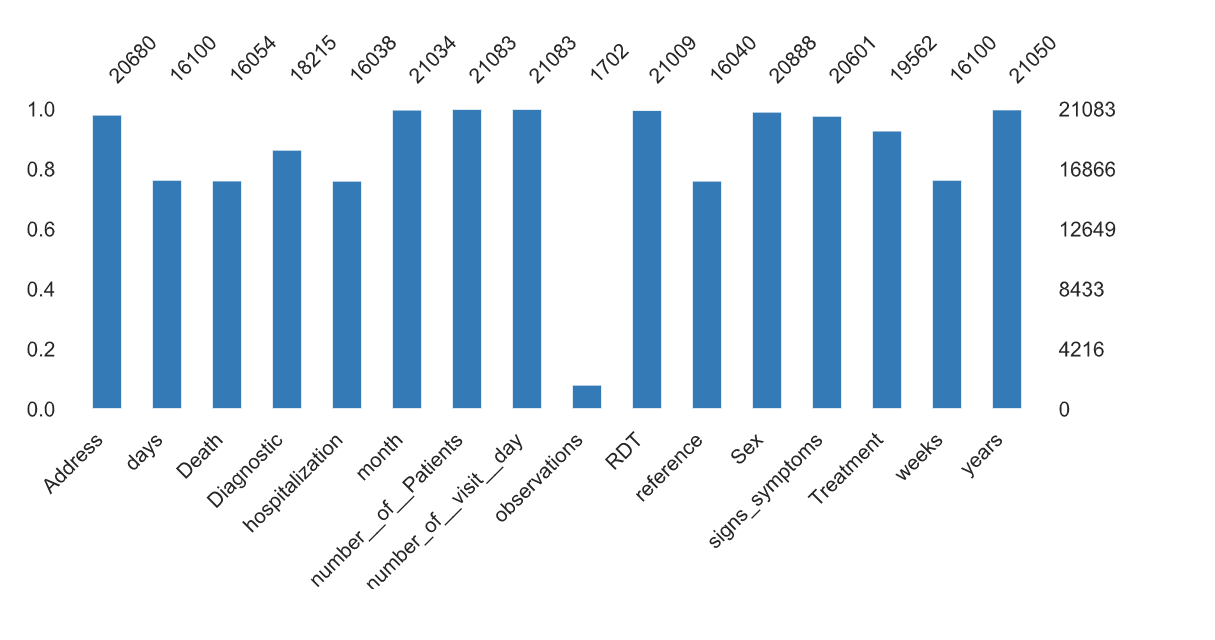
\includegraphics[width=.8\linewidth]{missing_values}
    \caption{Proportion of missing values per variable}
    \label{missing_values}
\end{figure*}

\subsubsection*{\textbf{Data preparation.}}
We have followed the same process as in 
\cite{mbaye2019towards} in order  to cleanse, normalize, impute, and balance information in our real datasets.  Firstly, the raw datasets come with lot of inconsistencies due to the way the information were originally collected within the health structures. Indeed information about patients are manually recorded in the majority of health structures in Senegal. 
Second, when we did an explanatory analysis of the set of real-world data, they have revealed that the datasets were not balanced  and come with missing values as mentioned above. We then used \emph{OpenRefine}\footnote{https://openrefine.org/} to first clean and normalize information in our datasets. After that, we resolved our problem of missing values and unbalanced datasets by respectively using a K-Nearest Neighbours based imputation algorithm and an oversampling of the minority class: for more details we defer the reader to \cite{mbaye2019towards}. Figure \ref{synthetic_data} summarizes the new characteristics of DT1 and DT2 after the data preparation step. 
\begin{table}[!ht]
\centering
\scriptsize
  \begin{tabular}{ccccccc}
    \toprule
    \multirow{2}{*}{\textbf{Dataset}} &
      \textbf{Variables}&\textbf{Observations}&
      \multicolumn{2}{c}{\textbf{Variables types}}& \multicolumn{2}{c}{\textbf{Classes}} \\
    & & & Numeric & Boolean & Malaria & not Malaria \\
    \midrule
    DT1 &16 & 61396 & 2 &  14& 30698&30698\\
    DT2 & 16 & 14336 & 2 & 14 & 7168&7168\\
    \bottomrule
  \end{tabular}
  \caption{Data characteristics after preparation step}\label{synthetic_data}
\end{table}

From DT1 and DT2 we built three news datasets DT3, DT4 and DT5 data sets as below.\\
 DT3: It is obtained by concatenating the DT1 and DT2 datasets. Thus it concerns 37,175 patients of which 9,837 are diagnosed positive for malaria.\\
DT4: It is obtained by considering the 16,092 patients in the DT2 data set (including 9,223 patients with malaria). Since this DT2 is unbalanced, we randomly selected 2354 patients who tested negative for malaria from the DT1 data set at the end of the rebalance. Thus it concerns 18,446 patients, 9,223 of whom are suffering from malaria.\\
DT5: is obtained by the over sampling of DT1 by the SMOTE method of python. This method consists first of dividing DT1 into two parts, one for training (train set) and the other for testing (test set). The train set being unbalanced, then we apply the SMOTE method to remedy it. Thus we obtain a new train set comprising 30,369 patients, half of whom tested positive for malaria.





% Experimentation and Results
\section{Experimentation and results}\label{experimentations}
We detail and analyze in the section the results of the experimentation we performed using the six ML algorithms presented in Section \ref{ml_algorithms} over the two real datasets described in Section \ref{datasets}. We start by presenting our experimentation setting.

% experimentation setting
\subsection{Experimentation Setting}
In this section data is available for applying classification algorithm. After model creation from training data, classification operation is performed on test data. 
All the performed tests have been done in the same machine and the same operating system. To test the performance of our six chosen ML algorithms, we relied on their Python implementations available through the scikit-learn library. Scikit-learn is an open source simple and efficient tool for predictive data analysis that implements most of the existing ML algorithms

Then some of the most important performance evaluation measures like accuracy, precision, sensitivity, specificity, F-measure and area under ROC curve are evaluated and compared. 
For the details about the description of each parameter of ML we refer to the official documentation of the implementation of these algorithms in scikit-learn7. Concerning the segmentation of both datasets for the training of our ML algorithms and their testing we have considered the stratified-5-fold cross-validation in classification model construction and efficiency evaluation. This method is very useful to handle data with an unbalanced class distribution, increases the validation of classification and prevents from random and invalid results.


% Results of the experiments
\subsection{Results of the experiments}

This section presents the results of the experimentation on each real dataset for each of the six classifiers. 
\subsubsection{Decision Tree}

Table 1  below shows the performance measures (precision, recall, F measure and precision) of the results of our Decision Tree classifier after experimentation on all our datasets. The observation shows that the best scores of our classifier are achieved on the datasets DT1, DT3 and DT5 which are 97.04\%, 80.86\% and 83.41\% respectively. Also AUC (Area Under the Curve) values are higher for these same datasets which are 0.78, 0.86 and 0.76 respectively. However, we note that the sensitivity values are higher than the specificity values on the datasets DT1 and DT5 so that they are substantially identical for the datasets DT2, DT3 and DT4. This means that DT is more inclined to predict as well whether a given patient has malaria or he doesn’t, on the datasets DT2, DT3 and DT4, while our classifier on the datasets DT1 and DT5 our classifier is only efficient in predicting whether a given patient has malaria. This same trend is observed on the F-scores which higher values varying between 0.91 and 0.98 on the datasets DT1, DT3 and DT5.

% Decision Tree
\begin{table}[!ht]
\centering
\begin{tabular}{*{7}{c}l r}
  \toprule
  \textbf{Datasets} & \textbf{Precision} & \textbf{Recall} & \textbf{F1-score}&\textbf{AUC} &\textbf{Score}&\textbf{Specificity}\\
   \midrule
  DT1 &0.97  & 1   & 0.98 & 0.78 & 97.04 & 0.05 \\
  DT2 & 0.59 &0.48 &0.48  &0.64  &63.01  &0.80\\
  DT3 &0.89  &0.85 &0.87  &0.86  &80.86  &0.69\\
  DT4 &0.68  &0.57 &0.62  &0.70  &65.60  &0.74\\
  DT5 &0.99  &0.84 &0.91  &0.76  &83.41  &0.58\\

  
    \bottomrule
\end{tabular}
\caption{Performances measures of DT over all datasets}\label{perf-measure-dt1}
\end{table}
\subsubsection{Random Forest}
The performance of the random forest varied throughout the study depending on the dataset, although overall it performed well as shown in Table 2. Notice that best accuracy are achieved by random forest classifier on the datasets DT1, DT2 and DT5 which are respectively 97.13\%, 80.86\% and 78.35\%. In contrast with the results obtained with the DT classifier, the Sensivity values are higher than specificity values on datasets DT1 and DT5 whereas the inverse is noticed on the dataset DT3. At the same time we note that these values are roughly identical on the datasets DT3 and D4
%Random Forest
\begin{table}[!ht]
\centering
\begin{tabular}{*{7}{c}l r}
  \toprule
  \textbf{Datasets} & \textbf{Precision} & \textbf{Recall} & \textbf{F1-score}&\textbf{AUC} &\textbf{Score} &\textbf{Specificity}\\
   \midrule
  DT1 &0.97 &1   &0.99 &0.81 &97.13& 0.07\\
  DT2 &0.63  & 0.34  &0.44&0.64&63.33& 0.85\\
  DT3 &0.89 &0.85 &0.87&087&80.86&0.70\\
  DT4 &0.68 &0.56&0.62&0.70&65.82&0.74\\
  DT5 &0.99 &0.84&0.91&0.76&78.35&0.60\\
  
  
    \bottomrule
\end{tabular}
\caption{Performances measures of RF over all datasets}\label{perf-measure-dt1}
\end{table}


%Logistic Regression
\subsubsection{Logistic Regression}

Logistic regression In table 3 we show the performance measures LR classifier experimented on our five datasets. We notice that our classifier have overall precision which are vary between 58\% and 98\%. 

\begin{table}[!ht]
\centering
\begin{tabular}{*{7}{c}l r}
  \toprule
  \textbf{Datasets} & \textbf{Precision} & \textbf{Recall} & \textbf{F1-score}&\textbf{AUC} &\textbf{Score}&\textbf{Specificity}\\
   \midrule
  DT1 &0.97 &1   &0.99 &0.79 &97.19&0.05 \\
  DT2 & 0.58 &0.36   &0.44&0.63&61.96&0.81\\
  DT3 &0.85 &0.88 &0.86&0.86&79.59&0.55\\
  DT4 &0.98 &0.56&0.92&0.70&65.82&0.72\\
  DT5 & 0.90&0.78&0.88&0.84&81.86&0.75\\
  
  
    \bottomrule
\end{tabular}
\caption{Performances measures of LR over all datasets}\label{perf-measure-dt1}
\end{table}
We observe that the higher precision is obtained with DT4 dataset while the corresponding score is equal to 65.82\% is the lowest of all other datasets. Also we notice that the LR presents homogeneous results on the DT3 dataset with an accuracy of 85\%, a sensitivity equal to 88\%, an F-score of 92\%, an AUC which is 0.86 and a score equal to 79.59\%. . We also note that the best AUC and the best F-score are obtained by LR on the DT3 dataset.
\subsubsection{Naives Bayes}
In contrast with the results above, NB classifier presents very heterogeneous performances regarding the performance measures used as shown in Table 4. In fact, we observe that the best precision is achieved on the dataset DT5 which is 99\%, although the best F-score and the higher accuracy are obtained on the dataset DT1 which are 0.99 and 97.13\% respectively and finally the best AUC is observed on the dataset DT3 which is 0.85. We also note that the best specificity is obtained on DT4 and varies between 0.65 and 0.70 (see appendices).
\begin{table}[!ht]
\centering
\begin{tabular}{*{7}{c}l r}
  \toprule
  \textbf{Datasets} & \textbf{Precision} & \textbf{Recall} & \textbf{F1-score}&\textbf{AUC} &\textbf{Score}&\textbf{Specificity}\\
   \midrule
  DT1 &0.97 &1   &0.99 &0.81 &97.13 &0.00\\
  DT2 & 0.60 &0.34   &0.43&0.63&62.86&0.83 \\
  DT3 &0.86 &0.87 &0.86&0.85&79.94&0.60\\
  DT4 &0.68 &0.59&0.63&0.70&65.63&0.73\\
  DT5 &0.99 &0.82&0.90&0.84&85.61&0.71\\
  
  
    \bottomrule
\end{tabular}
\caption{Performances measures of NB over all datasets}\label{perf-measure-dt1}
\end{table}
\subsubsection{Support Vector Machine}
%SVM

Table 5 shows the performance measures of the SVM classifier.
\begin{table}[!ht]
\centering
\begin{tabular}{*{7}{c}l r}
  \toprule
  \textbf{Datasets} & \textbf{Precision} & \textbf{Recall} & \textbf{F1-score}&\textbf{AUC} &\textbf{Score}&\textbf{Specificity}\\
   \midrule
  DT1 &0.97 &1   &0.99 &0.84 &97.13&0.00 \\
  DT2 &0.58  &0.05   & 0.09&0.62&62.86&0.97\\
  DT3 &0.57 & 0.86&0.86&0.85&79.94&0.64\\
  DT4 & 0.68&0.58&0.62&0.70&65.63&0.73\\
  DT5 &0.99 &0.86&0.92&0.80&85.61&0.62\\
    \bottomrule
\end{tabular}
\caption{Performances measures of SVM over all datasets}\label{perf-measure-dt1}
\end{table}
Table 1 shows the performance measures. The observation shows that the best score, precision and F1-score are obtained on the datasets DT1, DT3 and DT5. However the higher AUC and the best specificity are observer on the datasets DT1, DT3 and DT4.
%ANN
\subsubsection{Artificial Neural Nework}
The performance of the ANN varied throughout the study depending on the dataset, although overall it performed well. A large amount of initial effort was required to train and validate the model. Notice that best precision are achieved by ANN classifier on the datasets DT1, DT3 and DT5 which are respectively 97\%, 89\% and 99\%. While the higher AUC and the best scores are obtained on the datasets DT1 and DT3. The Sensivity values are higher than specificity values on datasets 
\begin{table}[!ht]
\centering
\begin{tabular}{*{8}{c}l r}
  \toprule
  \textbf{Datasets} & \textbf{Precision} & \textbf{Recall} & \textbf{F1-score}&\textbf{AUC} &\textbf{Score}&\textbf{Specificity}\\
   \midrule
  DT1 &0.97&1 &0.99   &0.84 &97.15&0.04  \\
  DT2 &0.59  &0.40   &0.48&0.65&62.86&0.80 \\
  DT3 &0.89 &0.85 &0.87&0.87&86.68&0.69\\
  DT4 &0.68 &0.58&0.62&0.70&0.70&0.75\\
  DT5 &0.99 &0.84&0.91&0.79&83.26&0.65\\ 
    \bottomrule
\end{tabular}
\caption{Performances measures of ANN over all datasets}\label{perf-measure-dt1}
\end{table}




% Conclusion
\section{Conclusion}\label{conclusion}


%
% ---- Bibliography ----
%
% BibTeX users should specify bibliography style 'splncs04'.
% References will then be sorted and formatted in the correct style.
%
\bibliographystyle{splncs04}
\bibliography{biblio}
%

=======
<<<<<<< HEAD
\renewcommand*{\familydefault}{\sfdefault}
\usepackage{tikz}
\usepackage{multirow}
\begin{document}
\pagestyle{headings}
\def\thepage{}

\begin{frontmatter}              % The preamble begins here.


%\pretitle{Pretitle}
\title{Prediction of Malaria with Machine Learning
Algorithms : An experimental Study}

\markboth{}{November 2020\hb}
%\subtitle{Subtitle}

\author[A]{\fnms{Oussseynou} \snm{MBAYE}%
\thanks{Corresponding Author: Book Production Manager, IOS Press, Nieuwe Hemweg 6B,
1013 BG Amsterdam, The Netherlands; E-mail:
bookproduction@iospress.nl.}},
\author[B]{\fnms{Mamadou Lamine } \snm{BA}}
and
\author[B]{\fnms{Alassane} \snm{SY}}

\runningauthor{O. MBAYE et al.}
\address[A]{ALioune Diop University of Bambey }
\address[B]{ALioune Diop University of Bambey}

\begin{abstract}
Still today, Malaria remains one of the most feared diseases in Sub- Saharan Africa and especially in Senegal. This is mainly due to inappropriate medical care support coupled with an often late and error-prone diagnosis from the medical staff. In addition, largely used diagnostic standards such as the Rapid Diagnosis Test is not fully reliable. With the development and increasing adoption of automated tools in the health field, machine learning applications might help medical actors in their decision-making process. In this paper, we propose an experimental study of six machine learning algorithms for the prediction of Malaria in Senegal. These algorithms aim at predicting whether or not a given patient suffers from Malaria based on his signs and symptoms. The performance of the algorithms have been extensively tested and evaluated over real data sets about patients in Senegal that suffer or not from Malaria. The algorithms are evaluated using four criteria: accuracy, Recall, F-measure, Precision and Specificity. The research has shown that there is not necessarily a single best classification tool, but instead the best performing algorithm will depend on the dataset to be analysed
\end{abstract}

\begin{keyword}

\end{keyword}
\end{frontmatter}
%\markboth{January 2020\hb}{January 2020\hb}
%\thispagestyle{empty}
%\pagestyle{empty}

% Introduction
\section{Introduction}\label{Introduction}
Malaria is a transmissible disease through the bites of infected female Anopheles mosquitoes. It comes with symptoms such as fever, headache, and chills in its early stage and can evolve to more severe health problems (severe anaemia, respiratory distress, etc.) often leading death. In 2019, the number of Malaria cases worldwide has been estimated to 229 millions. The number of deaths caused by Malaria has been approximatively estimated to 409 000 in 2019; the African area represents around 94\% of the reported malaria cases and deaths in 2019, thanks to the annual world Malaria report \cite{19WMR}. 

Over the past years, many efforts have been made by governmental and non governmental organizations (e.g. WHO) to eradicate Malaria in the world.  In the research field, many studies, aiming at understanding the disease from the Plasmodium mosquito point of view or proposing automated detection tools, have been conducted \cite{Ga19,Le74,ermert2011development,Hu17}. The Rapid Diagnostic Test (RDT) \cite{Hu17} is one of the most successful and prominent introduced tool to automatically predict whether or not a given patient suffers from Malaria. It relies on the detection of the presence of specific Plasmodium proteins, PfHRP2, pLDH
and aldolase in human blood. The RDT is largely used and adopted as a standard many Sub-saharan African countries such as Senegal. However, as proved in \cite{Hu17}, RDT is not fully reliable:  Section \ref{Methods} shows that the precision of RDT is about 90\% for datasets used in this study. Despite those advanced tools, Malaria is still a real public health in sub-Saharan African countries such as Senegal because of the lack of appropriate care support or late and error-prone detection of the disease.
Artificial intelligence is now recognized as a domain that may help medical actors in their decision-making process. \cite{mitchell1997machine, Ug1}  
 This paper proposes an  extensive comparative study of the most popular machine learning models for the task of Malaria prediction. The evaluated and compared ML algorithms are Naive Bayes (NB), Logistic Regression(LR),  Decision Tree(DT), Support Vector Machine(SVM) ,
 Random Forest(RF), and Artificial Neural Network(ANN). We conducted experiments on five datasets about patients living in Senegal. The raw
 datasets have been collected in different settings and contain clinical data such as sign, symptom and the diagnostic of the doctor.  The outcome of the RDT is also provided. Our main result is that Random Forest, Logistic Regression, Support Vector Machine with Gaussian kernel and Artificial Neural Network outperforms RDT and present very high precision in the Senegalese patient datasets.
The rest of the paper is organized as follows. We start by presenting the methods used in this work in section \ref{Methods}. In section \ref{results_discussion} details the results of the intensive experimentations conducted over various datasets. Finally, we conclude this paper in section \ref{conclusion}.


% Prediction Model
\newpage
\section{Methods}\label{Methods}
\subsection{Machine Learning algorithms in healthcare}
There are already some attempts to apply ML techniques for the prediction or a better understanding of various diseases, e.g. logistic regression has been tested in \cite{mbaye2019towards} for the prediction of Malaria and provides promising results.
\subsection{Datasets}
In order to carry out  our experiments in a real setting we have collected two real world datasets about patients living in Senegal. We describe each of them in the sequel.\\
\textbf{Data collection.} Our first dataset, that we  to refer to it as DT1, contains medical records about patients living in distinct places in Senegal. It has been collected in 2016 during the \textbf{Grand Magal of Touba}  which is one of the most popular religious event in Senegal. Such an event gathers every year several millions of persons that come from various areas around the country \cite{Ch17}.  During the event several fixed and mobile health points are set up to enable the examination and treatment of ill persons. The second dataset, denoted by DT2, has been collected by drawing our attention on medical records about patients living in the same area. We focused on the district of Diourbel,Thies and Fatick \footnote{https://en.wikipedia.org/wiki/Diourbel\_Region} where the prevalence of Malaria is very high and collected patient records from its different health structures. \\
\textbf{Data features.} Table \ref{raw_data} contains the main characteristic of each dataset. Some of these variables (also called features or attributes) include personal data about the patient, but also signs and symptoms(e.g. lack of appetite, tiredness, fever, cephalalgia, nausea,
arthralgia, digestive disorders, dizziness, chill, myalgia, diarrhea, and abdominal pain) of the patient reported by the doctor who treated this later. The other attributes describe clinical data such as information about the doctor's final diagnosis (the patient's disease), the outcome of the Rapid Diagnosis Test and the patient's status (i.e. admission, death or observation). For privacy reasons and certain restrictions in the use of the data, we have ignored patient personal data  during this study.
In addition, we can observe that  both datasets are unbalanced because the proportion of observations per class is largely unequal. As an example for dataset DT1 we have 614 observations in the first class and 5108 observation in the second class. Finally, we remarked that the precision of the Rapid Diagnosis Test is around 90\% for both datasets, meaning that the systematically performed RDT in Senegal is not fully reliable.
\begin{table*}[h]
\centering
  \begin{tabular}{cccccccc}
    \toprule
    \multirow{2}{*}{\textbf{Dataset}} &
      \textbf{Variables}&\textbf{Observations}&
      \multicolumn{2}{c}{\textbf{Variables types}}& \multicolumn{2}{c}{\textbf{Classes}} & \textbf{Precision of RDT}\\
    & & & Numeric & Boolean & Malaria & not Malaria \\
    \midrule
    DT1 &16 & 21083  & 2 &  14& 614&20469 & 90.23\% \\
    DT2 & 16 & 5809 & 2 & 14 & 5108&701 & 90.49\% \\
    \bottomrule
  \end{tabular}
  \caption{Raw Data characteristics}\label{raw_data}
\end{table*}

From DT1 and DT2 we built three news datasets DT3, DT4 and DT5 data sets as below.\\
\textbf{DT3:}  It is obtained by concatenating the DT1 and DT2 datasets. Thus it concerns 37,175 patients of which 9,837 are diagnosed positive for malaria.\\
\textbf{DT4:} It is obtained by considering the 16,092 patients in the DT2 data set (including 9,223 patients with malaria). Since this DT2 is unbalanced, we randomly selected 2354 patients who tested negative for malaria from the DT1 data set at the end of the rebalance. Thus it concerns 18,446 patients, 9,223 of whom are suffering from malaria.\\
\textbf{DT5:} is obtained by the over sampling of DT1 by the SMOTE method of python. This method consists first of dividing DT1 into two parts, one for training (train set) and the other for testing (test set). The train set being unbalanced, then we apply the SMOTE method to remedy it. Thus we obtain a new train set comprising 30,369 patients, half of whom tested positive for malaria.
\subsection{Machine Learning algorithms studies}
In the following we discuss about some of these methods.  Those algorithms are chosen among the most used ones in the health field according to studies\cite{de2018binary,tomar2013survey}.\\
\textbf{Decision tree (DT)}\cite{Ro05} is a supervised classifier which is obtained by recursively partitioning the labelled set of observations. It is one of the most adopted classifiers, thanks to its simplicity and its straightforward interpretation. For CART algorithms, hyperparameters are the impurity criteria (entropy and gini), the maximum depth, the minimum samples to split and the minimum samples at a leaf

% Random forest
Random Forest (RF) \cite{Be01}: RF is an ensemble approach built upon many decision tree classifiers. It is a supervised classifier which requires the same hyper parameters as DT, plus the number of trees to create and the random number of features to look at when splitting the labelled data during the training step \cite{Be01}.\\
% Naive Bayes
Naive Bayes classifier (NB): NB\cite{Ka17} is a\emph{supervised} machine learning algorithm, i.e. requires to be trained, used for classifying observations to given distinct classes based on \emph{input explanatory variables} (a.k.a feature or attribute).
It is a classification technique based on the well-known \emph{Bayes’ theorem}\footnote{https://en.wikipedia.org/wiki/Bayes\%27\_theorem} with strong and naive assumptions. It simplifies learning by assuming that features are independent of given class.\\
% Logistic Regression 
Logistic regression (LR: LR \cite{Ph88} is a statistical model used in the machine learning domain as a supervised classifier for binary classification \cite{uddin2019comparing}. 
It is based, in its basic form, on a logistic function to describe a binary dependent variable\cite{wang2014support,de2018binary} by considering as input 
qualitative or/and ordinal explanatory variables  in order to measure the probability of a given class label. \\
%Support Vector Machine
Support Vector Machine (SVM): SVM \cite{Ev01} is a supervised classification approach whose intuition is to represent input data in a space and to determine the optimal hyper-plane that divides that space in two regions depending on the targeted value.\\
% artificial neural networks
 Artificial Neural Network (ANN): ANN \cite{Me19} is a computational approach also referred to as a Connectionist System used in Machine Learning. ANNs are loosely modeled after the biological neural network in an attempt to replicate the way in which we learn as humans. Think of it as a computing system, structured as a series of layers, each layer consisting of one or several neurons. The types of the layers comprise \emph{input}, \emph{output} and \emph{hidden} layers \cite{anderson1972simple,raschka2015python}.
\subsection{Experimentation Setting}
In this section data is available for applying classification algorithm. After model creation from training data, classification operation is performed on test data. 
All the performed tests have been done in the same machine and the same operating system. To test the performance of our six chosen ML algorithms, we relied on their Python implementations available through the scikit-learn library. Scikit-learn is an open source simple and efficient tool for predictive data analysis that implements most of the existing ML algorithms.
For the details about the description of each parameter of ML we refer to the official documentation of the implementation of these algorithms in scikit-learn7. Concerning the segmentation of both datasets for the training of our ML algorithms and their testing we have considered the stratified-5-fold cross-validation in classification model construction and efficiency evaluation. This method is very useful to handle data with an unbalanced class distribution, increases the validation of classification and prevents from random and invalid results.
\subsection{Measurement} 
To evaluate the performance of every considered algorithm we have considered common measures of the accuracy of a prediction system that are \emph{Precision}, \emph{Recall}, \emph{F1-score}, \emph{True Positive Rate}, and
 \emph{False Positive Rate} on both datasets augmented with semi-synthetic datasets which are obtained after imputation in order to deal with missing values.
% Related work
\section{Results of the experiments}
Table \ref{raw_data1} presents the results of the experiments with the different algorithms on our data on Malaria. More specifically, Table 2 contains the precision, the recall, the specificity, the AUC mesure, the score and F-measure of each algorithm tested while Figure 1 shows their respective ROC curve.  
\begin{table}[h]
\begin{tabular}{|l|c|c|c|c|c|c|c|}
\hline
\cline{2-8}
 \textbf{ML ALgorithms} &  \textbf{Datasets} & \textbf{Precision} & \textbf{Recall} & \textbf{F1-score}&\textbf{AUC} &\textbf{Score}&\textbf{Specificity}\tabularnewline
\hline
\cline{2-8}
 &  DT1 &0.97  & 1   & 0.98 & 0.78 & 97.04 & 0.05 \\
\cline{2-8}
& DT2 & 0.59 &0.48 &0.48  &0.64  &63.01  &0.80\\
\cline{2-8}
& DT3 &0.89  &0.85 &0.87  &0.86  &80.86  &0.69\\
\cline{2-8}
& DT4 &0.68  &0.57 &0.62  &0.70  &65.60  &0.74\\
\cline{2-8}
\multirow{-4}{*}{ \textbf{Decision Tree}}&   DT5 &0.99  &0.84 &0.91  &0.76  &83.41  &0.58\\
\hline
\cline{2-8}
&DT1 &0.97 &1   &0.99 &0.81 &97.13& 0.07\\
\cline{2-8}
 & DT2 &0.63  & 0.34  &0.44&0.64&63.33& 0.85\\
 \cline{2-8}
 & DT3 &0.89 &0.85 &0.87&087&80.86&0.70\\
 \cline{2-8}
 & DT4 &0.68 &0.56&0.62&0.70&65.82&0.74\\
\cline{2-8}
\multirow{-4}{*}{ \textbf{Random Forest}}&   DT5 &0.99 &0.84&0.91&0.76&78.35&0.60\\
\hline
\cline{2-8}
&DT1 &0.97 &1   &0.99 &0.79 &97.19&0.05 \\
\cline{2-8}
 &DT2 & 0.58 &0.36   &0.44&0.63&61.96&0.81\\
 \cline{2-8}
  &DT3 &0.85 &0.88 &0.86&0.86&79.59&0.55\\
  \cline{2-8}
  &DT4 &0.98 &0.56&0.92&0.70&65.82&0.72\\
  \cline{2-8}
\multirow{-4}{*}{ \textbf{Logistic Regression}}&   DT5 & 0.90&0.78&0.88&0.84&81.86&0.75\\
\hline
\cline{2-8}
& DT1 &0.97 &1   &0.99 &0.81 &97.13 &0.00\\
 \cline{2-8}
  &DT2 & 0.60 &0.34   &0.43&0.63&62.86&0.83 \\
  \cline{2-8}
  &DT3 &0.86 &0.87 &0.86&0.85&79.94&0.60\\
  \cline{2-8}
  &DT4 &0.68 &0.59&0.63&0.70&65.63&0.73\\
  \cline{2-8}
\multirow{-4}{*}{ \textbf{Naive Bays}}&0.99 &0.82&0.90&0.84&85.61&0.71&0.71\\
\hline
\cline{2-8}
&DT1 &0.97 &1   &0.99 &0.84 &97.13&0.00 \\
\cline{2-8}
  &DT2 &0.58  &0.05   & 0.09&0.62&62.86&0.97\\
  \cline{2-8}
  &DT3 &0.57 & 0.86&0.86&0.85&79.94&0.64\\
  \cline{2-8}
 & DT4 & 0.68&0.58&0.62&0.70&65.63&0.73\\
 \cline{2-8}
 \multirow{-4}{*}{ \textbf{Support V Machine}}& DT5 &0.99 &0.86&0.92&0.80&85.61&0.62\\
 \hline
\cline{2-8}
&DT1 &0.97&1 &0.99   &0.84 &97.15&0.04  \\
\cline{2-8}
&  DT2 &0.59  &0.40   &0.48&0.65&62.86&0.80 \\
\cline{2-8}
 & DT3 &0.89 &0.85 &0.87&0.87&86.68&0.69\\
 \cline{2-8}
 & DT4 &0.68 &0.58&0.62&0.70&0.70&0.75\\
  \cline{2-8}
  \multirow{-4}{*}{ \textbf{ Artificial N Network}}&DT5 &0.99 &0.84&0.91&0.79&83.26&0.65\\ 
  \hline
\end{tabular}
\caption{Performances measures of our classifiers over all datasets}\label{raw_data1}
\end{table}

% Data Preparation
\subsection{Discussion}
In this study, the algorithms DT, RF, LR, NB, SVM and ANN were applied on five datasets concerning patients with or without malaria and living in regions of Senegal namely: Diourbel, Thies and Fatick. Indeed, in order to offer a new technique for diagnosing and predicting malaria, it is important to know the performance of those existing through our datasets.
Analysing in details the performance of our six classifiers across the five datasets, the results show that there is not necessarily a single best classification algorithm, but that the best performing algorithm will depend on the characteristics of the dataset to analyze. Indeed we notice that all the algorithms produce their best precision on the DT1, DT3, and DT5 data sets. These values, which reach 97\% at times, outperform the Rapid Diagnosis Test which is the standard diagnostic tool largely adopted in the healthcare system in Senegal.
\begin{figure}
\begin{tikzpicture}[scale=0.8]
 \centering
\begin{axis}[
    height=8cm, width=15.5cm,
    bar width=0.4cm,
    ybar,
    %ybar=5pt,% configures `bar shift'
    bar width=9pt,
    enlargelimits=0.15,
    legend style={at={(0.5,-0.15)},
    anchor=north,legend columns=-1},
    ylabel={\#AUC},
    symbolic x coords={{DT,RF,LR,NB,SVM,ANN}},
    xtick=data,
    %nodes near coords,
    nodes near coords align={vertical},
    ]
\addplot coordinates {(DT,0.78) (RF, 0.81) (LR,0.79)(NB, 0.81)(SVM,0.84)(ANN, 0.54)};
\addplot coordinates{(DT,0.64) (RF, 0.64) (LR,0.63)(NB, 0.63)(SVM,0.62)(ANN, 0.65)};
\addplot coordinates {(DT,0.86) (RF, 0.87) (LR,0.86)(NB, 0.85)(SVM,0.85)(ANN, 0.87)};
\addplot coordinates {(DT,0.70) (RF, 0.69) (LR,0.70)(NB, 0.69)(SVM,0.70)(ANN, 0.70)};
\addplot coordinates {(DT,0.76) (RF, 0.76) (LR,0.84)(NB, 0.84)(SVM,0.80)(ANN, 0.79)};
\legend{DT1,DT2,DT3,DT4,DT5}
\end{axis}
\end{tikzpicture}
\caption{Comparison of the ROC Curves of the classifiers on differents datasets}
\end{figure}
However, on these same datasets, the algorithms often present very low specificities, for example 0.05 on DT1. This shows that our best performing classifiers are only able to predict a single class: either the patient has malaria or he does not, but not in both spots. This is because the DT1 and DT3 datasets are very unbalanced. In fact in these datasets either the number of patients with malaria is greater than those who are not or the opposite is true. Furthermore, we note that on the DT2 and DT4 datasets all the algorithms present specificities and Sensivity that are significant and quite similar. Contrary to what is quoted a little above, on these datasets the algorithms are efficient on the prediction tasks of the two classes. Looking closely at the results in terms of precision, recall and F-measure we observe that the classifiers RF, LR, SVM and ANN generally outperform the others for each dataset. Indeed, for the dataset DT1, which contains observations on patients living in different regions of Senegal, these four classifiers have an accuracy of 99\%, a recall greater than 92\% and an F-measure greater than 95\%. We note the same trend with the DT2 dataset which contains observations on patients living in the same area in Senegal. It can also be noted that RF, LR, SVM and ANN have better precision than the rapid diagnostic test carried out and systematically used in the majority of health structures in Senegal. This observation remains true with DT4 which is a perfectly balanced dataset. In conclusion, it is very difficult or even impossible for us to say definitively which algorithm is more efficient for the task of predicting malaria, but the choice of this one will strongly depend on the choice of the data set. However, this study shows that our classification problem has been taken care of. A method integrating several models and various datasets is necessary

\begin{figure}[!h]
\subfigure[Precision values of compared classifiers on different datasets]{
\begin{tikzpicture}[scale=0.8]
 %\centering
\begin{axis}[
    height=8cm, width=6cm,
    bar width=0.4cm,
    ybar,
    %ybar=5pt,% configures `bar shift'
    bar width=9pt,
    enlargelimits=0.15,
    legend style={at={(0.5,-0.15)},
    anchor=north,legend columns=-1},
    ylabel={\#AUC},
    symbolic x coords={{DT,RF,LR,NB,SVM,ANN}},
    xtick=data,
    %nodes near coords,
    nodes near coords align={vertical},
    ]
\addplot coordinates {(DT,0.97) (RF, 0.97) (LR,0.97)(NB, 0.97)(SVM,0.97)(ANN, 0.97)};
\addplot coordinates{(DT,0.59) (RF, 0.63) (LR,0.58)(NB, 0.60)(SVM,0.58)(ANN, 0.59)};
\addplot coordinates {(DT,0.89) (RF, 0.89) (LR,0.85)(NB, 0.86)(SVM,0.57)(ANN, 0.89)};
\addplot coordinates {(DT,0.68) (RF, 0.68) (LR,0.98)(NB, 0.68)(SVM,0.68)(ANN, 0.68)};
\addplot coordinates {(DT,0.99) (RF, 0.99) (LR,0.90)(NB, 0.99)(SVM,0.99)(ANN, 0.99)};
\legend{DT1,DT2,DT3,DT4,DT5}
\end{axis}
\end{tikzpicture}
%\caption{Precision values of compared classifiers on different datasets}
}
\subfigure[Precison, F1-score, specificity values of the classifiers on DT1]{
\begin{tikzpicture}[scale=0.8]
\begin{axis}[
    height=8cm, width=6cm,
    bar width=0.4cm,
    ybar,
    %ybar=5pt,% configures `bar shift'
    bar width=9pt,
    enlargelimits=0.15,
    legend style={at={(0.5,-0.15)},
    anchor=north,legend columns=-1},
    ylabel={\#AUC},
    symbolic x coords={{DT,RF,LR,NB,SVM,ANN}},
    xtick=data,
    %nodes near coords,
    nodes near coords align={vertical},
    ]
\addplot coordinates {(DT,0.59) (RF, 0.63) (LR,0.58)(NB, 0.60)(SVM,0.58)(ANN, 0.59)};
\addplot coordinates{(DT,0.48) (RF, 0.44) (LR,0.44)(NB, 0.43)(SVM,0.09)(ANN, 0.48)};
\addplot coordinates {(DT,0.80) (RF, 0.85) (LR,0.81)(NB, 0.83)(SVM,0.97)(ANN, 0.80)};
%\addplot coordinates {(DT,0.68) (RF, 0.68) (LR,0.98)(NB, 0.68)(SVM,0.68)(ANN, 0.68)};
%\addplot coordinates {(DT,0.99) (RF, 0.99) (LR,0.90)(NB, 0.99)(SVM,0.99)(ANN, 0.99)};
\legend{Precision,F1-score,Specificity,DT4}
\end{axis}
%\caption{Precison, F1-score, specificity values of the classifiers on DT1}

\end{tikzpicture}
}
\end{figure}


%\begin{figure}
%\begin{tikzpicture}[scale=0.8]
% \centering
%\begin{axis}[
%    height=8cm, width=15.5cm,
%    bar width=0.4cm,
%    ybar,
%    %ybar=5pt,% configures `bar shift'
%    bar width=9pt,
%    enlargelimits=0.15,
%    legend style={at={(0.5,-0.15)},
%    anchor=north,legend columns=-1},
%    ylabel={\#AUC},
%    symbolic x coords={{DT,RF,LR,NB,SVM,ANN}},
%    xtick=data,
%    %nodes near coords,
%    nodes near coords align={vertical},
%    ]
%\addplot coordinates {(DT,0.59) (RF, 0.63) (LR,0.58)(NB, 0.60)(SVM,0.58)(ANN, 0.59)};
%\addplot coordinates{(DT,0.48) (RF, 0.44) (LR,0.44)(NB, 0.43)(SVM,0.09)(ANN, 0.48)};
%\addplot coordinates {(DT,0.80) (RF, 0.85) (LR,0.81)(NB, 0.83)(SVM,0.97)(ANN, 0.80)};
%%\addplot coordinates {(DT,0.68) (RF, 0.68) (LR,0.98)(NB, 0.68)(SVM,0.68)(ANN, 0.68)};
%%\addplot coordinates {(DT,0.99) (RF, 0.99) (LR,0.90)(NB, 0.99)(SVM,0.99)(ANN, 0.99)};
%\legend{Precision,F1-score,Specificity,DT4}
%\end{axis}
%\end{tikzpicture}
%\caption{Precison, F1-score, specificity values of the classifiers on DT1}
%
%\end{figure}
\section{Conclusion}
In this study, six classifiers using a wide variety of operating procedures have been extensively tested and compared over real world health datasets in order to evaluate their performance for the task of predicting the occurrence or not of Malaria in a patient knowing his signs and symptoms. The results obtained show that the algorithms RF, LR,
SVM with Gaussian kernel and ANN present the best performances in predicting the occurrence or not of Malaria. In addition those four algorithms outperform the Rapid Diagnosis Test which is the standard diagnostic tool largely adopted in the health system in
Senegal. This research has indicated that in practice there is no single best classification tool, but instead the best technique will on the characteristics of the dataset to be analysed. 
Future work consists in the study and the implementation of an ensemble method for predicting the occurrence or not of malaria based on the classifiers offering the best performances in our present study. But also to compare these performances with the ensemble methods for their validation



\begin{thebibliography}{99}
%\bibliography{IOS-Book-Article}
\end{thebibliography}
=======
%\renewcommand*{\familydefault}{\sfdefault}
\usepackage{tikz}

\def\hb{\hbox to 10.7 cm{}}

\begin{document}

\pagestyle{headings}
\def\thepage{}

\begin{frontmatter}              % The preamble begins here

%\pretitle{Pretitle}
\title{On the efficiency of Machine Learning Models in predicting Malaria using Sympt\^om Data}

\markboth{}{January 2020\hb}
%\subtitle{Subtitle}

\author{\fnms{Ousseynou} \snm{Mbaye}},
\author{\fnms{Mouhamadou Lamine} \snm{BA}
\thanks{Corresponding Author: Mouhamadou Lamine BA, LIMA, Universit\'e Alioune Diop,
BP.3400 Bambey, Senegal; E-mail: mouhamadoulamine.ba@uadb.edu.sn.}}
and
\author{\fnms{Alassane} \snm{SY}}

\runningauthor{O.Mbaye et al.}
\address{LIMA, Universit\'e Alioune Diop, Bambey, Senegal}
%\address[B]{Short Affiliation of Second Author and Third Author}

\begin{abstract}
Still today, Malaria remains one of the most feared diseases in Sub-Saharan Africa and especially in Senegal. This is mainly due to inappropriate medical care support coupled with an often late and error-prone diagnosis from the medical staff. In addition, largely used diagnostic standards such as the Rapid Diagnosis Test is not fully reliable. With the development and increasing adoption of automated tools in the health field, machine learning applications might help medical actors in their decision-making process. In this paper, we propose an experimental study of six machine learning algorithms for the prediction of Malaria in Senegal. These algorithms aim at predicting whether or not a given patient suffers from Malaria based on his signs and symptoms. The performance of the algorithms have been extensively tested and evaluated over real data sets about patients in Senegal that suffer or not from Malaria. The algorithms are evaluated using four criteria: accuracy, Recall, F-measure, Precision and Specificity. The research has shown that there is not necessarily a single best classification tool, but instead the best performing algorithm will depend on the dataset to be analysed.
\end{abstract}

\begin{keyword}
electronic camera-ready manuscript\sep IOS Press\sep
\LaTeX\sep book\sep layout
\end{keyword}
\end{frontmatter}
\markboth{January 2020\hb}{January 2020\hb}
%\thispagestyle{empty}
%\pagestyle{empty}

\section{Introduction}\label{intro}
Malaria is one amongst the most deadly disease in the world, especially in sub-saharan Africa countries such as Senegal.
Malaria is caused by parasitic single-celled microorganisms belonging to the Plasmodium group; it is an infectious
disease which is transmitted to human being through bites from infected female Anopheles mosquitoes. Someone who suffers
from  Malaria may present symptoms that typically include fever, tiredness, vomiting, and headaches. In its severe form,
the disease can cause yellow skin, seizures, coma or death.

\subsubsection{Studied problem and motivations.}
According to the last report \cite{Wh17}  about the propagation of Malaria disease around the world, published in November 2017 by the World international Health Organization (WHO in short),
 216 millions of cases have been reported in 2016. As a result, the number of cases has significantly increased when compared to the 211 millions of reported Malaria patients in 2016.
As for the number of death due to Malaria, it does not decrease between 2016 and 2017 (446.000 vs. 445.000) despite the huge effort made by governements
and non-governmental organization to improve healthcare services and the awareness strategies, especially in critical areas. 
When analyzing the statistics above in details, one can easily notice that the burden of the Africa region of the World 
international Health Organization is colossal. Indeed, 90\% of Malaria cases and 90\% of deaths due to the disease were located in this area in 2016.
More specifically, 80\% of the burden in terms of morbidity is distributed in fifteen countries, all located in Sub-saharan Africa except India. This demonstrates
that Malaria is a real flail in Sub-saharan Africa states and Senegal is not spared at all. We investigate in this study an efficient approach to predict, using machine learning, the occurence 
or not of Malaria when a patient has to be diagnosed. Given the patient signs and symptoms, as well as the result from the quick diagnosis test, our solution should be to 
automatically tell if she suffers from Malaria or not with a high accuracy.

Malaria is an acute problem in Senegal  due mainly to the lack of high quality healthcare services and well-formed
staffs able to perform accurate diagnosis of diseases that patients suffer from. Over the past years, the government with 
the help of international organizations have tried to eradicate Malaria by implementing various proactive and reactive solutions 
to fill the gap in terms of services and human resources. However, the mortality rate is still very high, e.g. in underserved areas,
areas without required healthcare needs, uneducated people, population with low income, etc. Most of these deaths cases are reported to be caused by inaccurate diagnosis, sometimes 
incomplete leading to a bad prediction of the exact type of Malaria.
On the other hand, Malaria occurence or complication can often occur during  popular events (for instance religious events such as the Grand Magal of Touba \cite{So17})
which gather thousands of persons from everywhere in the country during a short time period. During those popular events, non-permanent medical points are set in order
to assist and treat ill persons; the staff in a given health point might be formed sometimes by only volunteers without advanced medical skills. Each of these medical 
points might receive and treat hundreds of patients each day with some of them potentially suffering from Malaria. 
This appeals for the need of finding automated tools to help medical actors in their decision making process, and thereby to improve provided 
healthcare services.   

\subsubsection{Proposed diagnosis approach.}
In this paper we present first steps towards an efficient manner to automatically diagnosis Malaria occurence or not based on patient signs and symptoms,
and the outcome from the quick diagnosis test. We define our diagnosis task as a classical binary classification problem by considering two classes: \textquote{Malaria} and \textquote{not-Malaria}.
Given a patient data, our main goal is to properly find to which class the patient belongs. To solve this classification problem we rely on machine learning and use the logistic regression
function as the basis of our prediction approach. Machine learning has been largely used in several domains (e.g. Health Informatics  \cite{Du13}) for various purposes whereas logistic regression has demonstrated its efficiency when dealing with a binary classification problem. 
 
As an application scenario, we focus on predicting Malaria cases in Senegal. At this end, we use  a large volume of patient record dataset collected during the most popular religious event in Senegal from the different installed health points, namely more than twenty points that deadly receive hundreds of patients.
As an immediate result of this work, we introduce a data preparation pipeline in order to 
\begin{inparaenum}[(i)]
\item explore the dataset for profiling purpose;
\item only retain records related to Malaria;
\item clean and transform attributes, as well data values, into the extracted Malaria dataset; and 
\item impute missing values (there were lot of missing values in the collected health dataset as reported in Section\ref{data_prep}).
\end{inparaenum}
Such a data preparation pipeline has been realized using \emph{OpenRefine} (formely Google Refine) to perform various cleaning and profiling tasks on our raw atient dataset and \emph{missForest}, a robust
 algorithm for imputing  missing data of diverses types; see Section \ref{data_prep} for more details. 
Expermients on the real world patient dataset, augmenting with a semi-synthetic dataset, show promising performance results regarding the effectiveness of the proposed approach.

\subsubsection{Paper organization.}The remaining of the paper is organized as follows. We summarize the related work on data imputation and binary classification methods in Section \ref{related_work}.
In Section \ref{data_prep} we introduce a data preparation pipeline on the raw collected patient records for the prediction phase. 
We then present our prediction model for Malaria cases in Section \ref{prediction_model}.
Experiments and performance analysis  on the collected real-world dataset, as well as a semi-synthetic dataset,  are detailled in Section \ref{experimentation} before we conclude in Section \ref{conclusion}. 


\section{Related work}\label{related_work}
In this section, we summarize the sate-of-the-art research on Malaria in general, and in particular the
use of machine learning techniques to tackle the various aspects related to one of the 
major healthcare problems worldwide which is Malaria.

% Studies on Malaria
As it is well-known, Malaria is caused by the bite of the female Anopheles, the most dangerous of which
is Plasmodium falciparum. Many early works have been consequently focused on the study of the evolution and
the distribution of the responsible mosquito, mainly with the goal to detect or diagnosis the severity of the 
disease given an infected patient \cite{Fe03,Al09}. Recent research on Malaria have largely adopted machine learning
and showed its ability to solve various aspects of the disease. Most of these machine learning based techniques are 
based on the analysis of blood data obtained from high-definition microscopic screenshots as in \cite{Ku18}. The authors
in \cite{Ku18} propose an unsupervised learning algorithm that detects and determines the types of infected blood cells.
Used prediction approach consists of quantifying the amount of plasmodium parasites in a blood smear. In the same research intuition
of harnessing blood, the Jordan-Elman neural network classifier introduced in \cite{Ha15}, on the other hand, to quickly determine the occurrence 
of Malaria and its severity level as well: the neural network analyzes the features of the blood data of the patients.  
Still using ML, DIAZ et al. have proposed in \cite{Dia09} a semi-supervised algorithm enable to quantify and classify the 
erythrocytes infected by Malaria parasistes through microscopic images. The orginiality of this work comes from its usability
even in the presence of thin blood drandruff infected by falciparum Plasmodium for the quantification and the classificationi tasks.
Besides blood data, sign and symptom records were also used to study Malaria with ML methods. Indeed, decision trees based approach
has been proposed in Nigeria \cite{Ug10} to predict the occurrence of Malaria given diagnostic data. However a decision tree suffers 
from various limitations as a classifier. Indeed it can easily overfit or can be extremely sensitive to small pertubations in data for instance.
Even though we both rely on signs and symptoms, the prediction model in \cite{Ug10} differs from ours on numerous facets: our model is built upon
logistic regression and is trained using also inputs from the quick diagnosis test. In addition, we apply our method in the context of patients living in Senegal. 
An example of previous work that has used logistic regression is that of Farida et al. in \cite{Ad10}. The logistic regression is exploited
there for the selection of features in order to construct stable decision trees. The decision trees are then used to predict the severity
criteria of Malaria in the context of Afghanistan. 


In the same line of works applying machine learning, in \cite{Pr17}, Pranav et al. propose Malaria likelihood prediction model built on a deep reinforcement learning (RL) agent. 
Such a RL predicts the probability of a patient testing positive for Malaria using answers from questions about their household. In 
the presented approach the authors have also dealt with the problem of determining the right question to ask next as well as the length of the survey, dynamically.
Moreover, statistically enhanced rule-based classification model to diagnose malaria has been proposed in \cite{Bb16}. A corresponding prototype 
which incorporates the rules and statistical models have been implemented; the main goal of the study was to develop a statistical 
prototype to perform clinical diagnosis of malaria given its adverse effects on the overall healthcare, yet its treatment remains 
very expensive for the majority of the patients to afford.

To the best of our knowledge this is the first work in Senegal that attempts to provide a prediction model for identifying 
the occurrence of Malaria given patient data.  


\section{Review of evaluated ML algorithms}\label{ml_algorithms}
We considered and comparatively evaluated  the performance of six machine learning algorithms for the task of predicting Malaria appearance for patients living in Senegal. Those algorithms are chosen among the most used ones in the health field according to studies \cite{de2018binary,tomar2013survey}. In the following we briefly describe each of them.

% Naive Bayes
\textbf{ Naive Bayes classifier (NB) }\cite{Ka17} is a \emph{supervised} machine learning algorithm, i.e. requires to be trained, used for classifying observations to given distinct classes based on \emph{input explanatory variables} (a.k.a feature or attribute).
It is a classification technique based on the well-known \emph{Bayes’ theorem}\footnote{https://en.wikipedia.org/wiki/Bayes\%27\_theorem} with strong and naive assumptions.
It simplifies learning by assuming that features are independent of given class.

% Logistic Regression
 
\textbf{Logistic regression (LR)} \cite{Ph88} is a statistical model used in the machine learning domain as a supervised classifier for binary classification \cite{uddin2019comparing}. 
It is based, in its basic form, on a logistic function to describe a binary dependent variable\cite{wang2014support,de2018binary} by considering as input 
qualitative or/and ordinal explanatory variables  in order to measure the probability of a given class label. The greatest advantage  of the logistic regression
classifier is the fact that you can use continuous explanatory variables and it is easier to handle more than two explanatory variables simultaneously. One the other 
hand, the logistic regression is one of the most used multi-valued models in epidemiology.

% Decision Tree

\textbf{Decision tree (DT)} \cite{Ro05} is a supervised classifier which is obtained by recursively partitioning the labelled set of observations. It is one of the most adopted classifiers, thanks to its simplicity and its straightforward interpretation. For CART algorithms, hyperparameters are the impurity criteria (entropy and gini), the maximum depth, the minimum samples to split and the minimum samples at a leaf
 
% Random forest 

\textbf{Random Forest (RF)} \cite{Be01} is an ensemble approach built upon many decision tree classifiers. It is a supervised classifier which requires the same hyper parameters as DT, plus the number of trees to create and the random number of features
to look at when splitting the labelled data during the training step \cite{Be01}. 
%Support Vector Machine
 
\textbf{Support Vector Machine (SVM)} \cite{Ev01} is a supervised classification approach whose intuition is to represent input data in a space and to determine the optimal hyper-plane that divides that space in two regions depending on the targeted value.

% artificial neural networks

\textbf{An Artificial Neural Network (ANN)} \cite{Me19} is a computational approach also referred to as a Connectionist System used in Machine Learning. ANNs are loosely modeled after the biological neural network in an attempt to replicate the way in which we learn as humans. Think of it as a computing system, structured as a series of layers, each layer consisting of one or several neurons. The types of the layers comprise \emph{input}, \emph{output} and \emph{hidden} layers \cite{anderson1972simple,raschka2015python}.




\section{REAL PATIENT HEALTH DATASETS}\label{datasets}
In order to carry out  our experiments in a real setting we have collected two real world datasets about patients living in Senegal. We describe each of them in the sequel.

\subsubsection*{\textbf{Data collection.}} Our first dataset, that we  to refer to it as DT1, contains medical records about patients living in distinct places in Senegal. It has been collected in 2016 during the \textquote{Grand Magal of Touba}  which is one of the most popular religious event in Senegal. Such an event gathers every year several millions of persons that come from various areas around the country \cite{Ch17}.  During the event several fixed and mobile health points are set up to enable the examination and treatment of ill persons. The second dataset, denoted by DT2, has been collected by drawing our attention on medical records about patients living in the same area. We focused on the district of Diourbel,Thies and Fatick \footnote{https://en.wikipedia.org/wiki/Diourbel\_Region} where the prevalence of Malaria is very high and collected patient records from its different health structures. 

\subsubsection*{\textbf{Data features. }} Table \ref{raw_data} contains the main characteristic of each dataset in terms of number of recorded variables (mainly clinical features), number of observations, variable types, number of observations per class (Malaria or Not Malaria), and the precision of the Rapid Diagnosis Test. In details, values for seventeen variables have been extracted for each observation in both datasets; two variables are basically of numerical types while the remaining are Boolean. Some of these variables (also called features or attributes) include personal data about the patient, but also signs and symptoms of the patient reported by the doctor who treated this later. The other attributes describe clinical data such as information about the doctor's final diagnosis (the patient's disease), the outcome of the Rapid Diagnosis Test and the patient's status (i.e. admission, death or observation). For privacy reasons and certain restrictions in the use of the data, we have ignored patient personal data  during this study.
In addition, we can observe that the first dataset is larger than the second one (21083 observations versus 5809 observations). Moreover, both datasets are unbalanced because the proportion of observations per class is largely unequal. As an example for dataset DT1 we have 614 observations in the first class and 5108 observation in the second class. Finally, we remarked that the precision of the Rapid Diagnosis Test is around 90\% for both datasets, meaning that
the systematically performed RDT in Senegal is not fully reliable.

On the other hand,  Figure \ref{missing_values} shows that the raw datasets come with missing values for  some variables on given observations.
To resolve the problem of unbalanced datasets and data messness, we followed a data preparation pipeline in order to fit our datasets into the good format for our experimentation; we discuss about such a data preparation step next. 

\begin{table*}[!ht]
\centering
  \begin{tabular}{cccccccc}
    \toprule
    \multirow{2}{*}{\textbf{Dataset}} &
      \textbf{Variables}&\textbf{Observations}&
      \multicolumn{2}{c}{\textbf{Variables types}}& \multicolumn{2}{c}{\textbf{Classes}} & \textbf{Precision of RDT}\\
    & & & Numeric & Boolean & Malaria & not Malaria \\
    \midrule
    DT1 &16 & 21083  & 2 &  14& 614&20469 & 90.23\% \\
    DT2 & 16 & 5809 & 2 & 14 & 5108&701 & 90.49\% \\
    \bottomrule
  \end{tabular}
  \caption{Raw Data characteristics}\label{raw_data}
\end{table*}
%
\begin{figure*}[!ht]
    \centering
    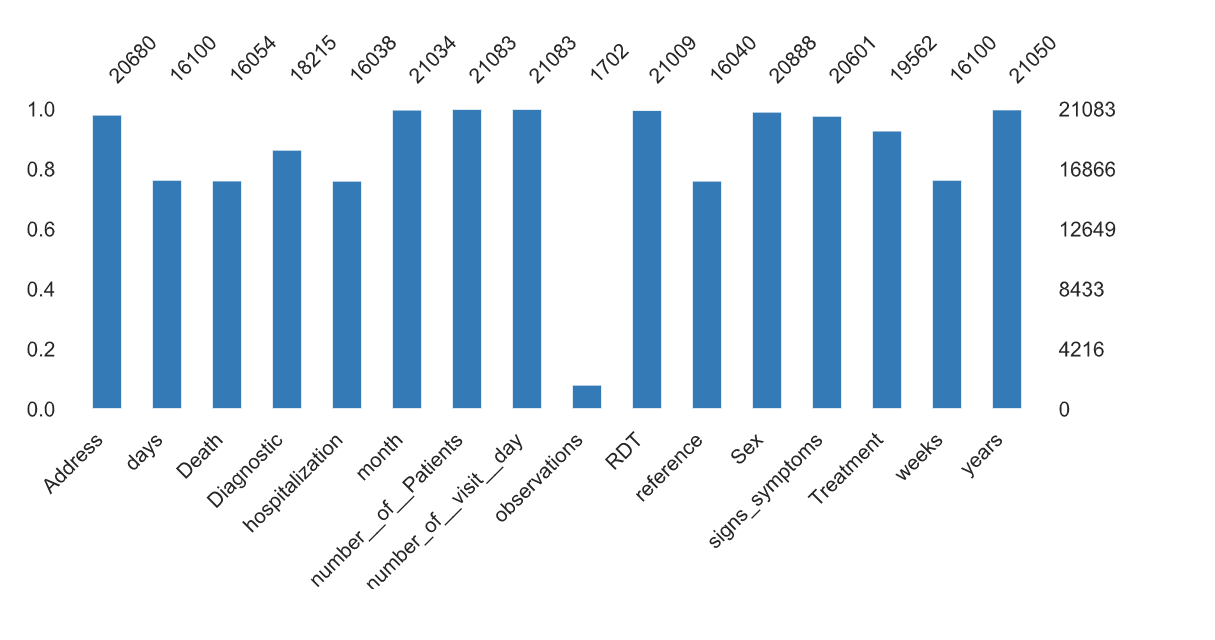
\includegraphics[width=.8\linewidth]{missing_values}
    \caption{Proportion of missing values per variable}
    \label{missing_values}
\end{figure*}

\subsubsection*{\textbf{Data preparation.}}
We have followed the same process as in 
\cite{mbaye2019towards} in order  to cleanse, normalize, impute, and balance information in our real datasets.  Firstly, the raw datasets come with lot of inconsistencies due to the way the information were originally collected within the health structures. Indeed information about patients are manually recorded in the majority of health structures in Senegal. 
Second, when we did an explanatory analysis of the set of real-world data, they have revealed that the datasets were not balanced  and come with missing values as mentioned above. We then used \emph{OpenRefine}\footnote{https://openrefine.org/} to first clean and normalize information in our datasets. After that, we resolved our problem of missing values and unbalanced datasets by respectively using a K-Nearest Neighbours based imputation algorithm and an oversampling of the minority class: for more details we defer the reader to \cite{mbaye2019towards}. Figure \ref{synthetic_data} summarizes the new characteristics of DT1 and DT2 after the data preparation step. 
\begin{table}[!ht]
\centering
\scriptsize
  \begin{tabular}{ccccccc}
    \toprule
    \multirow{2}{*}{\textbf{Dataset}} &
      \textbf{Variables}&\textbf{Observations}&
      \multicolumn{2}{c}{\textbf{Variables types}}& \multicolumn{2}{c}{\textbf{Classes}} \\
    & & & Numeric & Boolean & Malaria & not Malaria \\
    \midrule
    DT1 &16 & 61396 & 2 &  14& 30698&30698\\
    DT2 & 16 & 14336 & 2 & 14 & 7168&7168\\
    \bottomrule
  \end{tabular}
  \caption{Data characteristics after preparation step}\label{synthetic_data}
\end{table}

From DT1 and DT2 we built three news datasets DT3, DT4 and DT5 data sets as below.\\
 DT3: It is obtained by concatenating the DT1 and DT2 datasets. Thus it concerns 37,175 patients of which 9,837 are diagnosed positive for malaria.\\
DT4: It is obtained by considering the 16,092 patients in the DT2 data set (including 9,223 patients with malaria). Since this DT2 is unbalanced, we randomly selected 2354 patients who tested negative for malaria from the DT1 data set at the end of the rebalance. Thus it concerns 18,446 patients, 9,223 of whom are suffering from malaria.\\
DT5: is obtained by the over sampling of DT1 by the SMOTE method of python. This method consists first of dividing DT1 into two parts, one for training (train set) and the other for testing (test set). The train set being unbalanced, then we apply the SMOTE method to remedy it. Thus we obtain a new train set comprising 30,369 patients, half of whom tested positive for malaria.



\section{Experimentation and results}\label{experimentations}
We detail and analyze in the section the results of the experimentation we performed using the six ML algorithms presented in Section \ref{ml_algorithms} over the two real datasets described in Section \ref{datasets}. We start by presenting our experimentation setting.

% experimentation setting
\subsection{Experimentation Setting}
In this section data is available for applying classification algorithm. After model creation from training data, classification operation is performed on test data. 
All the performed tests have been done in the same machine and the same operating system. To test the performance of our six chosen ML algorithms, we relied on their Python implementations available through the scikit-learn library. Scikit-learn is an open source simple and efficient tool for predictive data analysis that implements most of the existing ML algorithms

Then some of the most important performance evaluation measures like accuracy, precision, sensitivity, specificity, F-measure and area under ROC curve are evaluated and compared. 
For the details about the description of each parameter of ML we refer to the official documentation of the implementation of these algorithms in scikit-learn7. Concerning the segmentation of both datasets for the training of our ML algorithms and their testing we have considered the stratified-5-fold cross-validation in classification model construction and efficiency evaluation. This method is very useful to handle data with an unbalanced class distribution, increases the validation of classification and prevents from random and invalid results.


% Results of the experiments
\subsection{Results of the experiments}

This section presents the results of the experimentation on each real dataset for each of the six classifiers. 
\subsubsection{Decision Tree}

Table 1  below shows the performance measures (precision, recall, F measure and precision) of the results of our Decision Tree classifier after experimentation on all our datasets. The observation shows that the best scores of our classifier are achieved on the datasets DT1, DT3 and DT5 which are 97.04\%, 80.86\% and 83.41\% respectively. Also AUC (Area Under the Curve) values are higher for these same datasets which are 0.78, 0.86 and 0.76 respectively. However, we note that the sensitivity values are higher than the specificity values on the datasets DT1 and DT5 so that they are substantially identical for the datasets DT2, DT3 and DT4. This means that DT is more inclined to predict as well whether a given patient has malaria or he doesn’t, on the datasets DT2, DT3 and DT4, while our classifier on the datasets DT1 and DT5 our classifier is only efficient in predicting whether a given patient has malaria. This same trend is observed on the F-scores which higher values varying between 0.91 and 0.98 on the datasets DT1, DT3 and DT5.

% Decision Tree
\begin{table}[!ht]
\centering
\begin{tabular}{*{7}{c}l r}
  \toprule
  \textbf{Datasets} & \textbf{Precision} & \textbf{Recall} & \textbf{F1-score}&\textbf{AUC} &\textbf{Score}&\textbf{Specificity}\\
   \midrule
  DT1 &0.97  & 1   & 0.98 & 0.78 & 97.04 & 0.05 \\
  DT2 & 0.59 &0.48 &0.48  &0.64  &63.01  &0.80\\
  DT3 &0.89  &0.85 &0.87  &0.86  &80.86  &0.69\\
  DT4 &0.68  &0.57 &0.62  &0.70  &65.60  &0.74\\
  DT5 &0.99  &0.84 &0.91  &0.76  &83.41  &0.58\\

  
    \bottomrule
\end{tabular}
\caption{Performances measures of DT over all datasets}\label{perf-measure-dt1}
\end{table}
\subsubsection{Random Forest}
The performance of the random forest varied throughout the study depending on the dataset, although overall it performed well as shown in Table 2. Notice that best accuracy are achieved by random forest classifier on the datasets DT1, DT2 and DT5 which are respectively 97.13\%, 80.86\% and 78.35\%. In contrast with the results obtained with the DT classifier, the Sensivity values are higher than specificity values on datasets DT1 and DT5 whereas the inverse is noticed on the dataset DT3. At the same time we note that these values are roughly identical on the datasets DT3 and D4
%Random Forest
\begin{table}[!ht]
\centering
\begin{tabular}{*{7}{c}l r}
  \toprule
  \textbf{Datasets} & \textbf{Precision} & \textbf{Recall} & \textbf{F1-score}&\textbf{AUC} &\textbf{Score} &\textbf{Specificity}\\
   \midrule
  DT1 &0.97 &1   &0.99 &0.81 &97.13& 0.07\\
  DT2 &0.63  & 0.34  &0.44&0.64&63.33& 0.85\\
  DT3 &0.89 &0.85 &0.87&087&80.86&0.70\\
  DT4 &0.68 &0.56&0.62&0.70&65.82&0.74\\
  DT5 &0.99 &0.84&0.91&0.76&78.35&0.60\\
  
  
    \bottomrule
\end{tabular}
\caption{Performances measures of RF over all datasets}\label{perf-measure-dt1}
\end{table}


%Logistic Regression
\subsubsection{Logistic Regression}

Logistic regression In table 3 we show the performance measures LR classifier experimented on our five datasets. We notice that our classifier have overall precision which are vary between 58\% and 98\%. 

\begin{table}[!ht]
\centering
\begin{tabular}{*{7}{c}l r}
  \toprule
  \textbf{Datasets} & \textbf{Precision} & \textbf{Recall} & \textbf{F1-score}&\textbf{AUC} &\textbf{Score}&\textbf{Specificity}\\
   \midrule
  DT1 &0.97 &1   &0.99 &0.79 &97.19&0.05 \\
  DT2 & 0.58 &0.36   &0.44&0.63&61.96&0.81\\
  DT3 &0.85 &0.88 &0.86&0.86&79.59&0.55\\
  DT4 &0.98 &0.56&0.92&0.70&65.82&0.72\\
  DT5 & 0.90&0.78&0.88&0.84&81.86&0.75\\
  
  
    \bottomrule
\end{tabular}
\caption{Performances measures of LR over all datasets}\label{perf-measure-dt1}
\end{table}
We observe that the higher precision is obtained with DT4 dataset while the corresponding score is equal to 65.82\% is the lowest of all other datasets. Also we notice that the LR presents homogeneous results on the DT3 dataset with an accuracy of 85\%, a sensitivity equal to 88\%, an F-score of 92\%, an AUC which is 0.86 and a score equal to 79.59\%. . We also note that the best AUC and the best F-score are obtained by LR on the DT3 dataset.
\subsubsection{Naives Bayes}
In contrast with the results above, NB classifier presents very heterogeneous performances regarding the performance measures used as shown in Table 4. In fact, we observe that the best precision is achieved on the dataset DT5 which is 99\%, although the best F-score and the higher accuracy are obtained on the dataset DT1 which are 0.99 and 97.13\% respectively and finally the best AUC is observed on the dataset DT3 which is 0.85. We also note that the best specificity is obtained on DT4 and varies between 0.65 and 0.70 (see appendices).
\begin{table}[!ht]
\centering
\begin{tabular}{*{7}{c}l r}
  \toprule
  \textbf{Datasets} & \textbf{Precision} & \textbf{Recall} & \textbf{F1-score}&\textbf{AUC} &\textbf{Score}&\textbf{Specificity}\\
   \midrule
  DT1 &0.97 &1   &0.99 &0.81 &97.13 &0.00\\
  DT2 & 0.60 &0.34   &0.43&0.63&62.86&0.83 \\
  DT3 &0.86 &0.87 &0.86&0.85&79.94&0.60\\
  DT4 &0.68 &0.59&0.63&0.70&65.63&0.73\\
  DT5 &0.99 &0.82&0.90&0.84&85.61&0.71\\
  
  
    \bottomrule
\end{tabular}
\caption{Performances measures of NB over all datasets}\label{perf-measure-dt1}
\end{table}
\subsubsection{Support Vector Machine}
%SVM

Table 5 shows the performance measures of the SVM classifier.
\begin{table}[!ht]
\centering
\begin{tabular}{*{7}{c}l r}
  \toprule
  \textbf{Datasets} & \textbf{Precision} & \textbf{Recall} & \textbf{F1-score}&\textbf{AUC} &\textbf{Score}&\textbf{Specificity}\\
   \midrule
  DT1 &0.97 &1   &0.99 &0.84 &97.13&0.00 \\
  DT2 &0.58  &0.05   & 0.09&0.62&62.86&0.97\\
  DT3 &0.57 & 0.86&0.86&0.85&79.94&0.64\\
  DT4 & 0.68&0.58&0.62&0.70&65.63&0.73\\
  DT5 &0.99 &0.86&0.92&0.80&85.61&0.62\\
    \bottomrule
\end{tabular}
\caption{Performances measures of SVM over all datasets}\label{perf-measure-dt1}
\end{table}
Table 1 shows the performance measures. The observation shows that the best score, precision and F1-score are obtained on the datasets DT1, DT3 and DT5. However the higher AUC and the best specificity are observer on the datasets DT1, DT3 and DT4.
%ANN
\subsubsection{Artificial Neural Nework}
The performance of the ANN varied throughout the study depending on the dataset, although overall it performed well. A large amount of initial effort was required to train and validate the model. Notice that best precision are achieved by ANN classifier on the datasets DT1, DT3 and DT5 which are respectively 97\%, 89\% and 99\%. While the higher AUC and the best scores are obtained on the datasets DT1 and DT3. The Sensivity values are higher than specificity values on datasets 
\begin{table}[!ht]
\centering
\begin{tabular}{*{8}{c}l r}
  \toprule
  \textbf{Datasets} & \textbf{Precision} & \textbf{Recall} & \textbf{F1-score}&\textbf{AUC} &\textbf{Score}&\textbf{Specificity}\\
   \midrule
  DT1 &0.97&1 &0.99   &0.84 &97.15&0.04  \\
  DT2 &0.59  &0.40   &0.48&0.65&62.86&0.80 \\
  DT3 &0.89 &0.85 &0.87&0.87&86.68&0.69\\
  DT4 &0.68 &0.58&0.62&0.70&0.70&0.75\\
  DT5 &0.99 &0.84&0.91&0.79&83.26&0.65\\ 
    \bottomrule
\end{tabular}
\caption{Performances measures of ANN over all datasets}\label{perf-measure-dt1}
\end{table}




\section{Conclusion}\label{conclusion}






\bibliographystyle{vancouver}
\bibliography{../biblio}

>>>>>>> 7c1cec024806f0122dbd3ebada2b3244dc9de7ab
>>>>>>> c5f4a12... Mise a jour Method
\end{document}
